\chapter{Introduction}

Log files are commonly inspected by system administrators and developers to detect suspicious behaviors and diagnose failure causes. Since size of log files grows fast, thus making manual analysis impractical, different automatic techniques have been proposed to analyze log files. Unfortunately, accuracy and effectiveness of these techniques are often limited by the unstructured nature of logged messages and the variety of data that can be logged.

KLFA is a tool that automatically analyzes log files and retrieves important information to identify failure causes. KLFA automatically identifies dependencies between events and values in logs corresponding to legal executions, generates models of legal behaviors and compares log files collected during failing executions with the generated models to detect anomalous event sequences that are presented to users.

Experimental results show the effectiveness of the technique in supporting developers and testers to identify failure causes.

kLFA has been described in \cite{Cotroneo:LogFileAnalysis:SOQUA:2007} and
\cite{Mariani:ISSRE:2008}.

Figure~\ref{fig:approach} shows the three steps of the technique,
while Figure~\ref{fig:modelInference} focus on the model generation.
Detailed information about the technique can be found
in~\cite{Mariani:ISSRE:2008}.

Following chapters describe for every step of the technique the
tools involved and give examples of the usage of the tools.

\begin{figure*}[ht!]
    \begin{center}
        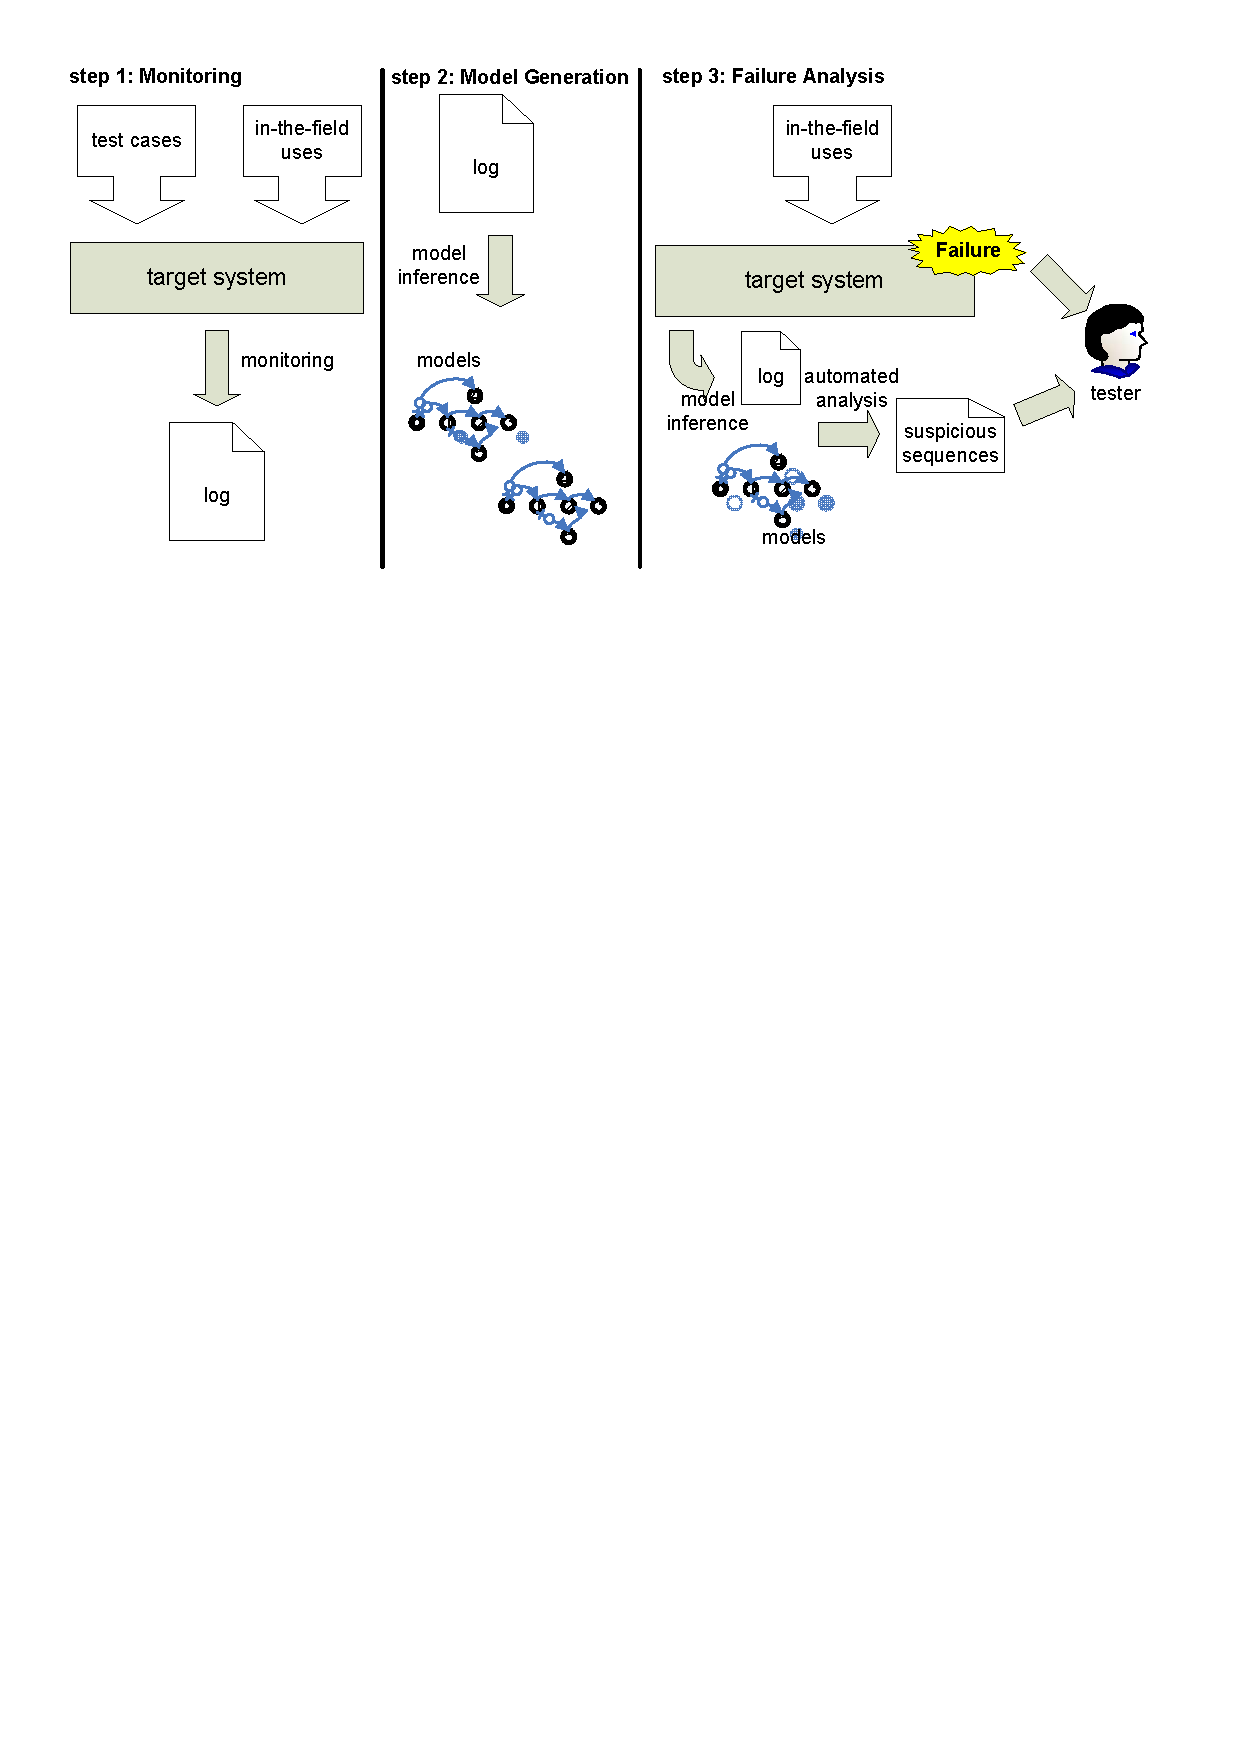
\includegraphics[width=12cm]{images/approach}
    \end{center}
    \caption{Automated log analysis.} \label{fig:approach}
\end{figure*}

\begin{figure*}[ht!]
    \begin{center}
        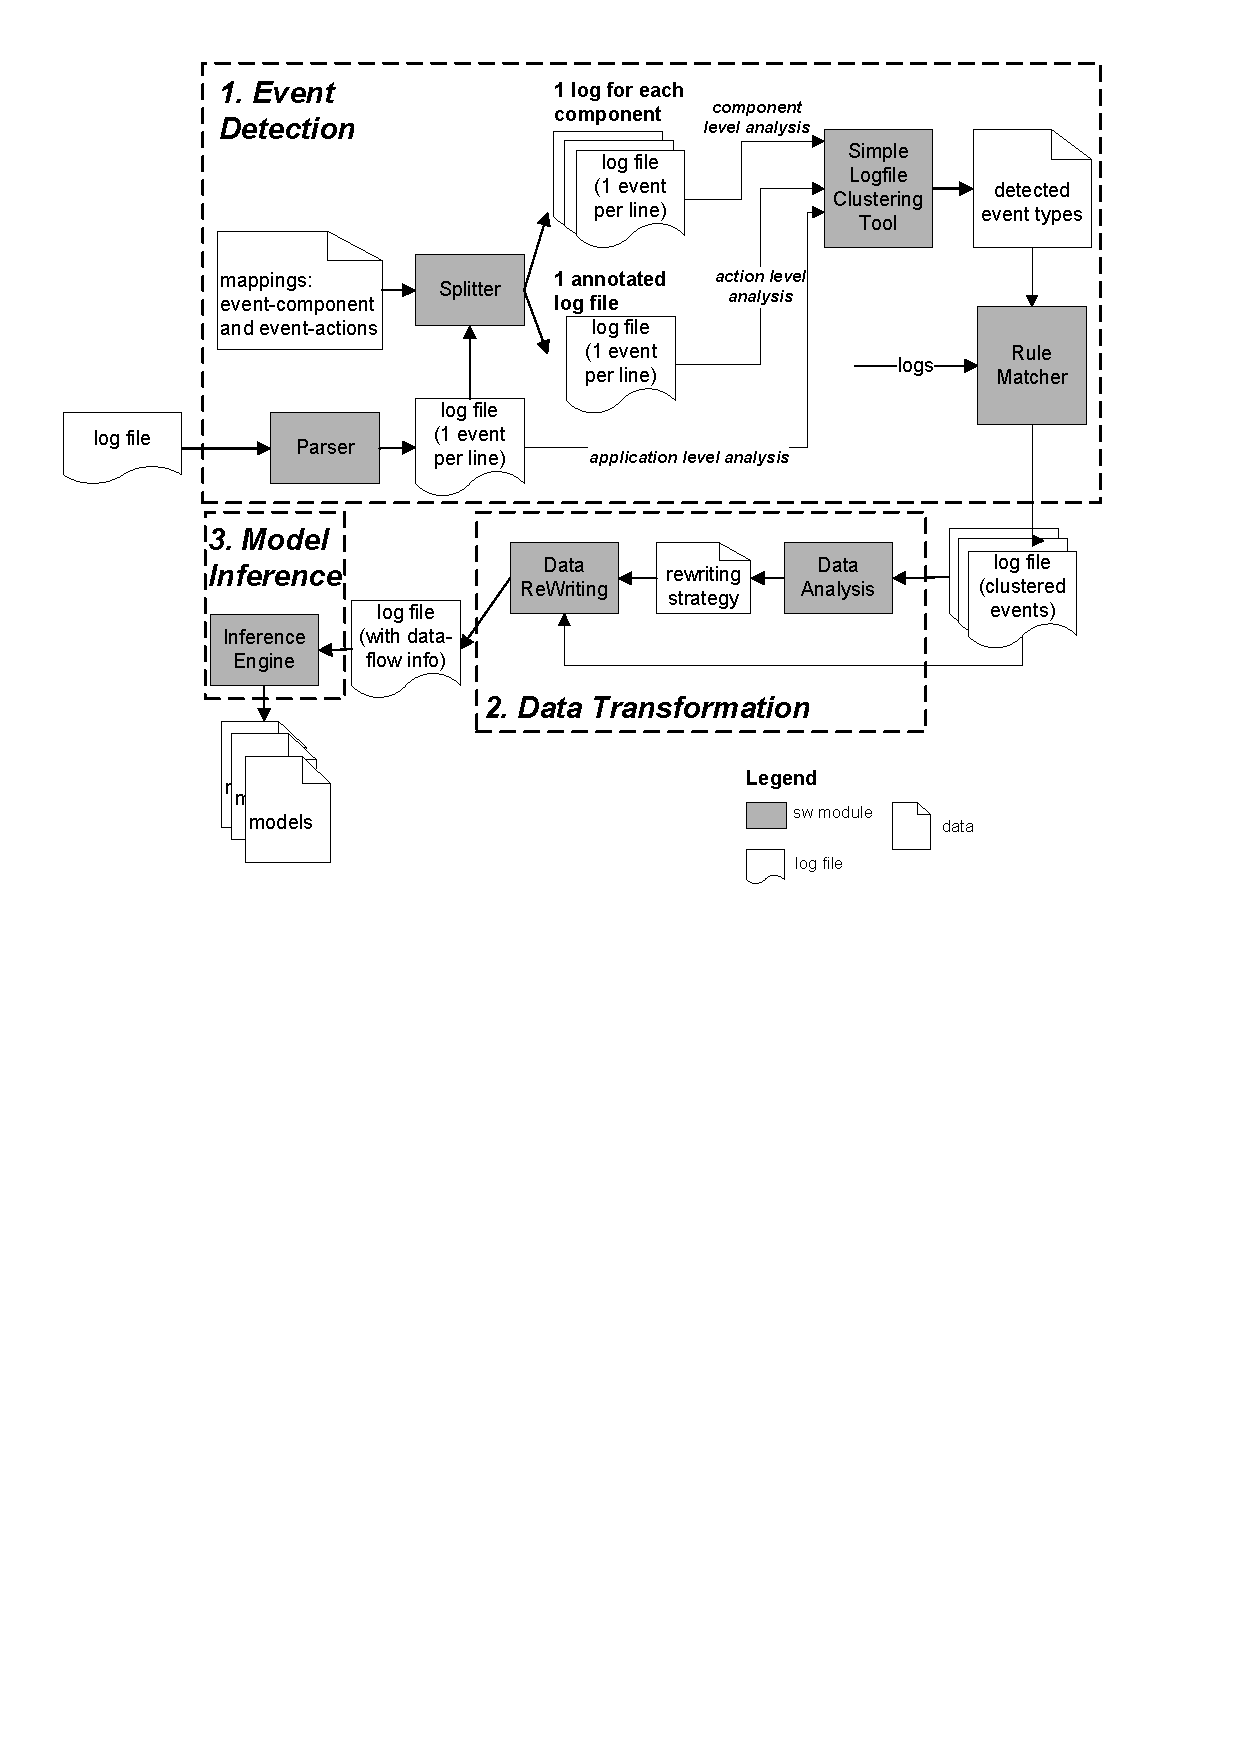
\includegraphics[width=12cm]{images/approach2}
    \end{center}
    \caption{Model generation.} \label{fig:modelInference}
\end{figure*}

